%!TEX root = ../LastNameI-[RnD-MT]Report.tex

\chapter{Approach}
\label{Approach}
%\begin{itemize}
%	\item What are the problems specific to the solver.
%	\item what does singularity mean in this case.
%	\item There are various places where the chain could be singular
%	\item What are their impacts? Chain cannot satisfy the constraint, diferent levels of interpretation(matrix rank, cannot invert)
%	\item Why are we interested in some decompositions, why investigate on projection.
%	\item Why are we interested in this use case. 
%	\item What do we want to achieve(exploit, avoid) - usecase.
%	\item How do u realize this with solver.
%	\item Why is this not sufficient.
%\end{itemize}
%The "section 2" describes the complete functionality of the Popov-Vereshchagin solver. According to the current implementation of the solver, it does not provide
%%%%%%%old version %%%%%%%%
%This chapter summarizes the methodology involved in detecting singularities early and efficiently. The solutions proposed are specific to the Popov-Vereshchagin constrained hybrid dynamics solver. Initial discussion focuses on difficulties in detecting the singularities specific to the solver. The later part of the chapter enunciates on numerical considerations and analysis which have been performed, for the approach. The chapter further provides information about the algorithmic level detection and finally the implementation and lessons learned.

%%%%%new%%%%%%%%%%
\section{Overview}
By definition singularity in manipulators can be defined as the state in which the end effector is incapable of moving in particular direction regardless of its movements in joints. They can also be defined on the level of forces as the configuration of manipulator achieved when force applied on the end effector does not produce any torque in the joints. There could be two situations of concern as mentioned earlier (refer section \ref{Motivation}) depending on the task performed by the robot. In few cases when the tasks are handled on the level of motions i.e., via velocities or accelerations, the necessity is that to avoid such singular configurations. Contrarily, when singularities are evaluated on the level of forces, then there are certain tasks for which we could exploit singularity. 

The main advantage of Popov Vereshchagin solver is that the cartesian acceleration, external forces and feedforward torques can be given as input task specifications. There are two main reasons to infer that the kinematic chain reaches singular configuration. The first one is that the kinematic chain when not be able to generate desired task specifications. The other reason is that the task constraints mentioned at end effector are not independent of each other \cite{shakhimardanov2015composable}. This means that different task specifications can be specified together and have can be conflicting to each other. The above reasons motivate the approach taken for the detection of singularities. 


%The \cite{shakhimardanov2015} mentions the implementation for the above but fails to check the conditions for the manipulator being in singularity.
%"Section 2" describes complete working of the solver
%As mentioned in "section 2", the main functionality of the solver is to handle the task constraints or specifications and minimize the gauss function to resolve them thus producing control commands. 

%But a detailed explanation is not provided. suggest that the solution to these above cases of can be handled by weighted pseudo inverse method "where singularity values will be checked by values closer to zero:-edit is not appropriate\cite{Buss2004}. The joint forces obtained through this method solves for acceleration constraints by weighting the Lagrange multiplier/ magnitude of constraint forces or the cartesian acceleration of the end effector \cite{shakhimardanov2015}. The solver has to be extended to determine singularities early and efficiently within the recursions, considering the above reasons as motivation.
%\section{Considerations }
As mentioned earlier in section \ref{Problem statement}, the requirement is to find an early and efficient detection for singularities i.e.\ to be able to detect the singularities earlier in the initial sweeps of the solver and also to find a decomposition technique which is computationally less expensive than the existing one. The current implementation of the Popov Vereshchagin solver lacks to check for the ill conditions of the kinematic chain being in singular configuration. There are certain insights for the approach which have been derived from \cite{shakhimardanov2015composable}. The overall approach can be outlined as backtracking the detection mechanism within the solver. 


This chapter summarizes the procedure involved in detecting singularities
early and efficiently. The solutions proposed are specific to the Popov-Vereshchagin Constrained hybrid dynamics solver. Initial discussion focuses on difficulties in identifying the singularities particular to the solver. The latter part of the chapter enunciates on the mathematical considerations necessary for producing an efficient solution . Then the chapter outlines on the implementation and hypothesis performed on the level of algorithm and finally, the limitations of the methodology.
%The authors have previously been significant contributors to the solver.
% In-order to detect singularity early in the sweeps, the necessity is to figure out where the singularity has first occurred or in which joint can we see them
\section{Solver specific singularities}
%Details of the solver. Traditional approach for singularity. The jacobian is hidden, how would you build the jacobian, cartesian end effector velocity is jacobian * joint velocity. The contribution of unit joint velocity to the end effector. The manipulator jacobian influence the end effector velocity. After building the jacobian you can determine the rank of the matrix(Jacobian) using svd. Why should I build up jacobian and analyze the rank of it and not use it(analyze it if we dont need it). Is there any other approach . Where could be mathematical singularities, if we divide by zero. Where all the inverses, D is always positive non zero scalar and cannot be singular. The other is Linv. Can it be trouble. What does it mean. what does it come from. Azamat reasoning, can do it. Svd gives us some information, can we make it more efficient by looking into other elements.
%Why does l have to be full rank to satisfy the constraints. What is the link

This section explains in detecting singularities which rely on the dynamic primitives available within the solver.

The Popov Vereshchagin is a hybrid dynamics solver which is derived from an optimization problem, and does not possess Jacobian matrix as a result, hence the traditional methods do not apply. Solution to the traditional approach can be obtained by building up the manipulator Jacobian for all the joints. Further analyzing on rank of the Jacobian following Singular value decomposition technique. However, this analysis does not contribute any insight on the early or efficient detection process within the solver. As the solver relies on matrices related to robot dynamics. This further initiates the need to explore other approach mechanisms. 


Within the solver, there are specific matrices related to robot dynamics which indicate mathematical singularity. This can be seen in the inward sweep of the algorithm (see line \ref{alg:P}) and in while determining the magnitude of constraint forces (see line \ref{alg:balance}) where the matrices are being inverted. These matrices are analyzed to provide further inputs to the detection mechanism. Referring to line \ref{alg:P} where term D is always a positive non zero scalar value indicating the sum of the joint inertia and joint rotor and thus indicates that the matrix is non singular and always invertible. The next step involves numerical examination of the constraint coupling matrix $\mathcal{L}$ (see line \ref{alg:balance}) in order to check if the matrix is always invertible. The constraint coupling matrix is a symmetric matrix as are all its prior contributors (refer inward sweep in section \ref{comprehensivesolver}) and is inverted during the calculation of magnitude of constraint forces, which forms the core part to be analyzed. 
%During the inward sweep, the algorithm keeps a track of the amount of acceleration energy which is generated by the unit constraint forces in a $m\times m$ constraint coupling matrix, where $m$ is the number of constraints. 
 
%Thus by backtracking the cause from 
The mathematical indication of the kinematic chain not being able to achieve the desired task specification can be indicated through $\mathcal{L}$ being singular. 
%Also in order to invert the $\mathcal{L}$ matrix it requires at least 'm' degrees of freedom in joints during every update in the inward sweep which are needed to generate 'm' constraint forces. Thus $\mathcal{L}$ matrix can attain singular configuration.

%The authors in \cite{shakhimardanov2015composable} indicate numerical considerations which have been made on the constraint coupling matrix $\mathcal{L}$ .. The further analysis is obtained by deriving certain information from the SVD of $\mathcal{L}$  matrix. There are evaluations or analysis which are also explored on other elements for the efficient and early detection process. 
 
 
%According to the traditional approach for singularity detection, in-order to provide an unique solution to the inverse kinematics equation, iterative methods using Jacobian inversion method have been proposed earlier. Jacobian within the solver can be defined as a matrix providing information about contribution of the unit joint velocities to the end effector (see line \ref{alg:velocity}). Solution to the traditional approach can be obtained by building up the manipulator Jacobian for all the joints. Further analyzing on rank of the Jacobian following Singular value decomposition technique. However, this analysis does not contribute any insight on the early or efficient detection process. This further initiates the need to explore other approach mechanisms. 


%Mathematically, singularity can be defined for example as a real function $1/x = 0$ where it is singular at $x=0$ and can explode to $\pm \infty$ where the function has not been defined \cite{unmentioned source-wikipedia}.
%The expression in the solver indicating the constraint coupling matrix is a symmetric matrix and also every previous term in the sweep which contributes to 'L' matrix is symmetric\cite{shakhimardanov2015}. This is be useful scenario for rank revealing decomposition.
%	During every recursion of matrix update, it adds a matrix of rank one. The calculation begins with a zero matrix. In order to invert the 'L' matrix it requires atleast 'm' degrees of freedom which are needed to generate 'm' constraint forces. The 'L' matrix can attain singular configuration. 
%Later the compositions of projections and transformations in equation \ref{alg:I_a} and \ref{alg:I_A2} can be analyzed for further detection in sweeps.\color{blue}"explained further".\color{black}
	%This could be mainly due to two reasons firstly the kinematic chain when not be able to generate desired task specifications(\color{blue}Equation ..).\color{black}The other reason is that the task constraints mentioned at end effector are not independent of each other\cite{shakhimardanov2015}
%	The svd of L matrix provides non negative values singular values of L matrix as the diagonal elements of sigma matrix. The singular values which belong to the null space of the L matrix are zero. If the manipulator is reaches singular configuration then the positive sigma values reduce and when they reach complete singular configuration then they become zero. Using this information, lead us to identify the direction of task constraints which cannot be satisfied.
%First may be explain math of the rank one update and then include a new line in the algorithm LL and LD compute them by doing LLlambdai and LDlambdai. Algorithmic level is trivial if you know math. Is there a link to physics or not. Matrices represent something from physical world. svd on matrix, there is no relation to physics. 
\section{Singularity analysis at the base}
\label{Numerical considerations}
%he naive way of solving the system of equations at the base; (ii) how this can help to identify the rank and thus singularities; (iii) what are matrix decompositions (maybe this is even part of the SOA?); (iv) how/why could matrix decompositions help here; (v) what are rank-one updates of matrix decompositions; and (vi) how/why can they help here?
%* The propagation of L is not always a rank-one update! What are the conditions?


As mentioned in the previous section, the issues are specific to the constraint coupling matrix and needs to be analyzed mathematically. There are naive approaches which can contemplate the detection process on an algorithmic level. The determination of rank of matrices in concern will already provide certain hints to the further problem solving. In the original algorithm, to solve the equations calculating $\nu$ at the base (see section \ref{comprehensivesolver}), the SVD over $\mathcal{L}$ matrix is performed. As we are aware that the $\mathcal{L}$ will lose rank when the robot has lesser DOF's than required to achieve task and is not able to generate the desired unit constraint forces. Thus merely by determining if the number of nonzero singular values during the SVD of $\mathcal{L}$ will provide the information on singularity. 

\section{Singularity analysis during the inward sweep}
The further steps necessitated in further early detection within the sweeps. By backtracking the inverted constraint coupling matrix to the generation of constraint coupling matrix forms the next step in the process (see line \ref{alg:L_i}). One such procedure, is by performing rank one update over matrix decompositions. However, in this scenario, it is necessary to find a decomposition technique which can satisfy certain properties of matrix $\mathcal{L}$. The recursion of $\mathcal{L}$ matrix begins with a positive semi definite (zero matrix), and every recursive update is symmetric. Thus, the decomposition should be able to handle the symmetricity and positive semi definite matrices in-order for the rank one updates to be possible. The other properties are that the decompositions should be rank revealing. The decomposed matrix should in-turn help in solving the linear equation at the base. The decomposition should also be computationally less expensive than the existing (SVD). 

The table \ref{Decomposition Techniques} provides a comparison of different matrix factorizations and the properties they can handle. The main comparisons are performed over LDL, SVD, QR and RRQR, UTV and VSV. 


	\begin{table}[h]
			\caption{Comparison of properties handled by different decompostions}
			\label{Decomposition Techniques}
		\renewcommand{\arraystretch}{3}
		\resizebox{1.0\textwidth}{!}{%
			\begin{tabular}{|l|l|l|l|l|l|l|l|l|}
				\hline
				\textit{\textbf{Properties}}              & \textit{\textbf{Sub-properties}}              & \multicolumn{7}{l|}{\textit{\textbf{Decompositions}}}                                                 \\ \hline
				&                                               & \textbf{LDL} & \textbf{LU} & \textbf{QR} & \textbf{SVD} & \textbf{RRQR} & \textbf{UTV} & \textbf{VSV} \\ \hline
				\textbf{Rank one update}                  & \textbf{Handle positive semi definite matrix} &    \checkmark          &             &             &     \checkmark         &    \checkmark \cite{hong1992rank}           &              &    \checkmark \cite{hansen2001computing}          \\ \hline
				\textbf{}                                 & \textbf{Exploits symmetric shape}             &   \checkmark           &   \checkmark          &             &              &      \checkmark         &              &   \checkmark           \\ \hline
				\textbf{Rank revealing}                   & \textbf{}                                     &              &    \checkmark         & \checkmark            &    \checkmark          &     \checkmark          &  \checkmark            &              \\ \hline
				\textbf{Computational complexity}         &  \textbf{}                                     &   $O(n^2)$           &   $O(nm^{2})$          &           &  $O(n^2)$            &               &   $O(mn^{2})$ \cite{gu1996efficient}      &              \\ \hline
%				\textbf{Numerical Stability}              & \textbf{}                                     &              &             &             &              &               &              &              \\ \hline
				\textbf{Ability to solve linear equation} & \textbf{}                                     &   \checkmark           &             &  \checkmark             &  \checkmark            &               &              &  \checkmark            \\ \hline
				\textbf{Unique decomposition}             &  \textbf{}                                     &    \checkmark          &  not always           &   \checkmark          &              &               &     unknown         &   unknown           \\ \hline
			\end{tabular}%
		}\renewcommand{\arraystretch}{2}
	
	\end{table}

Refer section \ref{algebra} for decomposition techniques and their uses.
These properties are essential inorder to provide an efficient detection process. As we can see the LDL decomposition is able to perform rank one update efficiently, satisfying all of the properties listed. The drawback of LU decomposition is that it does not handle positive semi definite matrices. Though RRQR satisfies all the properties, the computational complexity is greater than in the current implementation (SVD). UTV and VSV decompositions were looked into as they satisfied the rank one update conditions, but could not extract much information regarding the computational complexity and numerical stability.
%For the decomposition to perform an efficient rank one update, there are certain conditions in prior which are necessary to be considered. The sole purpose of rank one updates is that they allow faster and cheaper matrix inversions. 

From the above analysis on decomposition techniques, it is seen that the rank one updates through LDL decomposition satisfies all the prior conditions to perfrom an efficient rank one update.  Within the inward sweep of the algorithm (see algorithm1 \ref{alg1}) line \ref{alg:L_i} where it indicates that the recursion begins with a zero matrix and for every recursion it adds a rank-1 symmetric update which is rank revealing. Thus the authors in \cite{shakhimardanov2015composable} suggest the possibility of rank revealing LDL decomposition to provide an efficient decomposition which is presented in \cite{sentana1999econometric}. If solved using the above mentioned method then on finally reaching the base segment, the magnitude of constraint forces ($\nu$) can easily be determined as the matrix of constraint coupling matrix is in its decomposed form, which remains with solving for the linear equation in the form $Ax = b$.

%\par
%The detection of singularity on a algorithmic level can be performed using certain naive approaches. As discussed in the issues which are specific to the solver, the core analysis is performed on the constraint coupling matrix L. Some of the naive procedures are to obtain the rank of the matrix in concern which forms the initial steps in the detection process. 
\section{Rank one update of LDL decomposition}
As mentioned in \ref{Numerical considerations} when arriving at the base segment the numerical decomposition procedure should allow solving a linear set of equations \cite{shakhimardanov2015composable}. This section gives detailed explanation of the numerical approach involved in solving constraint coupling matrix efficiently.



The LDL decomposition of the positive semi definite constraint coupling matrix gives:
\begin{equation}
\mathcal{L}= \mathcal{L}_{L} . \mathcal{L}_{D} . \overline{\mathcal{L}}_{L}
\end{equation}
where $\mathcal{L}$ is a lower triangular matrix and $\mathcal{L}_{D}$ is the diagonal matrix. %This decomposition holds good in various applications \cite{sentana1999econometric}. 
The constraint coupling matrix is updated by a symmetric matrix of rank one to:
\begin{equation}
\overline{\mathcal{L}} = \mathcal{L} + \alpha.zz^{T}
\label{rankone:L}
\end{equation}
where $\alpha$ is a scalar value and z is a $n\times1$ vector. This equation can be compared to the line \ref{alg:L_i} and rewritten as :
\begin{equation}
\overline{\mathcal{L}} = \mathcal{L}_{i+1} + (A_{i+1}^T S_{i+1}D^{-1}_{i+1} S_{i+1}^T A_{i+1})
\label{alg:L}
\end{equation}


On comparing equations \ref{rankone:L} and \ref{alg:L} we see that $\alpha$ is same as $1/D$ as it a scalar value, $A_{i+1}^T S_{i+1}$ can be compared to z and similarly the transpose. In the original algorithm (see line \ref{alg:L_i}) the minus sign indicates the algorithm is computing the reaction force to the constraint forces \cite{bryunixonline}. The sign change to positive in equation \ref{alg:L} indicates the calculation of actual forces to constraint forces. To calculate the reaction forces again, it is possible by inverting the magnitude of constraint forces at the base (see algorithm \ref{alg2} line \ref{init}).

 
With the given decomposition, exploiting the decomposed factors of $\mathcal{L}$ in-order to obtain $\overline{\mathcal{L}}_{L}$, $\overline{\mathcal{L}}_{D}$ and $\overline{\mathcal{L}}_{L}$ which are efficient rank one update factors. The algorithm (refer appendix)proposed by \cite{sentana1999econometric} is provided as a slight modification to one of the methods in \cite{gill2007methods} in-order to account for $\alpha$ $>$ 0 when $\mathcal{L}$ is positive semi definite. 



\begin{algorithm}[H] \label{alg2}
		\Begin{
			$\mathcal{L}_{N} = 0$ \\
			\vspace{1mm}
			{// Inward sweep}\\
			\For{$\mathbf{i \ =  \ N-1  \ \ to \  \ 0}$}{
				refer lines \ref{alg:sum_inertia} - \ref{alg:U_i} from original algorithm \ref{alg1}\\
				$\alpha = \frac{1}{D}$, $w = A_{i+1}^T S_{i+1}$\; \label{alg:alpha}
				\vspace{2mm}
				${\mathcal{L}_i = \mathcal{L}_{i+1} + A_{i+1}^T S_{i+1}D^{-1}_{i+1} S_{i+1}^T A_{i+1}}$\; \label{alg:L_ii}
				\vspace{1mm}
				%			    // Perform rank one update \\[1mm]
				$\mathcal{L}^{'}_{L},\mathcal{L}^{'}_{D} = rank\_one\_update(\mathcal{L}_{L},\mathcal{L}_{D},\alpha,w)$\;\label{alg:rankone}
			}
			
			\vspace{1mm}
			%// Balance of acceleration energy at the base (\{0\} link)\\
			$A = \mathcal{L}_{0}, x = -\nu, b = b_{N} - A^{T}_{0}\ddot{X}_{0} - U_{0}$ \label{init}\\
			$\mathcal{L}D\mathcal{L}^{T}x = b$ \\
			$D\mathcal{L}^{T}x= forwardsubstitution(\mathcal{L},b) = y$ \\
			$\mathcal{L}^{T}x = D^{-1}y = z$ \\
			$x = backwardsubstitution(\mathcal{L}^{T},z)$ \\
			%			//forward substitution\\[1mm]
			%			$\mathcal{L}^{'}_{L} y = b_{N}$ \;
			%			//backward substitution\\[1mm]
			%			$\mathcal{L}^{'}_{L} x = y $ \;
			%			//Linear system of equation at the base\\[1mm]
			%			${\mathcal-{L}_0 \nu + A_0^T \ddot{X}_0 - U_0 = b_N}$\; \label{alg:balance}
			\vspace{1mm}
		}
		\caption{Extension to inward sweep in Popov Vereshchagin for efficient singularity detection}
	\end{algorithm}
%As explained in \ref{solver section}, the equation \ref{} indicates that despite these vectors having different physical units, the value will be the same. This can be helpful in detecting if the desired task constraints have been achieved or not.
%The singular value decomposition of L matrix provides non negative singular values as the diagonal elements of sigma matrix. The singular values which belong to the null space of the L matrix are zero. The unit constrained force matrix is taken as input by the user. The rank of these two matrices can be calculated to detect if the task constraint is satisfied or not. 
 %Run time analysis.
 %If the manipulator is reaches singular configuration then the positive sigma values reduce and when they reach complete singular configuration then they become zero. Using this information, lead us to identify the direction of task constraints which cannot be satisfied.
 %In the Vereshchagin solver, the task specification is specified in the unit constrained force matrix which indicates that the kinematic chain can be subjected to both linear and angular constraints. 
% Why did we begin with rank of matrix (Unit constrained force - sigma matrix)
%Factors that need to be considered in-order to detect  
%\section{Numerical considerations}
%As mentioned in \cite{shakhimardanov2015} the authors suggest a weighted pseudo inverse solution, by weighting either $\nu$ the magnitude of constrained forces or $\ddot{X}$ the desired end effector accelerations, which will in-turn approximate the acceleration constraints which are desired. The problem in these cases is the computational complexity which will be $O(n^3)$ where n is the number of constraints. The authors also suggest rank revealing decomposition, since it adds symmetric update in every recursion but the practical implementation is not available in the current implementation. If it is solved using the above mentioned method then finally on reaching the base segment, the value of $\nu$ can easily be determined as the matrix of constraint coupling matrix is in its decomposed form, which remains with solving for the linear equation in the form $Ax = b$.
%\newpage
%\section{Issues specific to solver}
%What are the consequences of solver being in singularity.
%The solver specific singularity can have the below listed effects on the kinematic chain. They are:
%\begin{enumerate}
%	\item The kinematic chain not being able to resolve the task constraints.
%	\item The kinematic chain provided with conflicting task constraints. 
%	\end{enumerate}
%\begin{enumerate}
%	\item Mathematically in the solver, there are certain naive approaches which could provide solution to the above problem. By detecting the rank of the matrix in concern. 
	%\item The matrices which are of concern are the unit constrained matrix , sigma(singular values) matrix(SVD decomposition of constraint coupling matrix)
%	\item If the task constraint is not achievable then the 
%\item The constraint coupling matrix is a symmetric matrix and is inverted during the calculation of magnitude of constraint forces, which forms the core part to be analyzed. The reason is , in the current implementation solves the least square equation using SVD. When kinematic chain is in singular configuration, the system of least square equations are underdetermined. This can also be interpreted as the decrease in rank of the matrix. There can be infinite number of solutions, hence the system becomes redundant. In such cases, the matrix is a non-square matrix and hence cannot be inverted. In our case, it is the constraint coupling matrix, and hence cannot be inverted.

%\item Also in the current implementation, Since the Moore-Penrose pseudoinverse, calculates the inverse of the L matrix and the singular values are reciprocated, this is used to obtain the inverse differential kinematic solution, "it is clear that singularities impose a serious hindrance, and even their vicinity is marked by unacceptably high joint velocities in the minimum-norm solution". We needed to avoid the inverse of L which is hugely composed matrix and hence reduce the computation expensiveness. 
%\item The next stage of analysis involved in reducing
%\begin{equation}
%A = U\Sigma V^{T}
%\end{equation}
%\item Our goal is to solve for the least squares equation $Ax = b$ at the base. 
%\end{enumerate}

%singularities and velocities, singularities and inverse.
%We begin by analyzing the solver to identify impact on kinematic chain when in singular configuration. The equations which could be affected by the singular configuration and help with the identification
%\section{Extension of Popov Vereshchagin Solver for singularity}

%\section{Decompositions techniques- Mathematical core}
%As discussed in \cite{shakhimardanov2015} previously the constraint coupling matrix is updated by symmetric elements in every recursion. Thus the authors suggest the possibility of rank revealing decomposition. The current implementation of the solver, does not handle this. But if it is solved using the above mentioned method then on finally reaching the base segment, the magnitude of constraint forces ($\nu$) can easily be determined as the matrix of constraint coupling matrix is in its decomposed form, which remains with solving for the linear equation in the form $Ax = b$.
 %As seen in table \ref{Decomposition techniques} there is a comparison being made between different properties which a decomposition technique should handle. For the decomposition to perform rank one update, there are certain conditions in prior which should considered. The rank one updates are mainly considered as they allow faster and cheaper matrix inversions. The matrix recursion of L matrix begins with a positive semi definite (zero matrix), and every recursive update is symmetric. Thus, the decomposition should be able to handle the symmetricity and positive semi definite matrices, inorder for the rank one updates to be possible symmetric update in every recursion and also rank revealing. The decomposed matrix should inturn help in solving the linear equation at the base. The decomposition should also be computationally less expensive than the current implementation. 
% \par
% The different matrix factorizations we looked into are LDL, SVD, QR, RRQR, UTV, VSV etc. These factorizations likely handled the requirements of our problem statement. 
%Handle positive semi definite,
%Symmetric shape exploit,
%Rank one update,
%Rank revealing,
%Computational complexity,
%Numerical Stability,
%Decomposition techniques 4 or 5 , LDL/Cholesky, SVD, LU, QR, RRQR, may be tick them and reference to the papers which indicate them.
%"http://simbaforrest.github.io/blog/2016/03/25/LDLT-for-checking-positive-semidefinite-matrix-singularity.html" Refer this link. 

% Please add the following required packages to your document preamble:
% \usepackage{booktabs}

% Please add the following required packages to your document preamble:
% \usepackage{lscape}
%\begin{sidewaystable}
% Please add the following required packages to your document preamble:
% \usepackage{graphicx}
% \usepackage{lscape}
%\begin{sidewaystable}

\section{Algorithmic level extension for singularity detection}
This section explains in detail the evaluation on the level of algorithm for detecting singularities. 

%There are certain naive techniques which can contemplate the detection process on an algorithmic level. However, they are not efficient. This initiated the necessity for efficient identification mechanism on the solver.


%The analysis begins with the constraint calculation (see line \ref{alg:balance}) of the constrained hybrid solver. 
As mentioned in section \ref{Numerical considerations} the initial investigation is performed on constraint coupling matrix $\mathcal{L}$. Also as discussed in sections \ref{Approach} and \ref{Numerical considerations}, for a faster and numerically efficient matrix inversion, the algorithm performs rank one symmetric update in every recursion of sweep. This has been depicted on the level of algorithm as an extension to the inward sweep \ref{alg2}. In lines \ref{alg:alpha}, \ref{alg:L_ii} it is shown that the $\alpha$ which is a scalar value is given the value of $1/D$. Further performing LDL decomposition on $\mathcal{L}$ will result in decomposed factors which are updated using rank one update as in \ref{alg:rankone}. Thus at the base the linear equation is easily solvable using forward and backward substitution.


Based on the criteria of run time complexity we analyze two decomposition techniques LDL and SVD inorder to measure the expensiveness of their operations. Firstly we evaluate the run time behavior of LDL decomposition technique. The rank one update performed through this decomposition will yield with a complexity of $O(n.nc^2)$ i.e.\ $O(nc^2)$ where nc is the no of constraints and n is the number of segments. This decomposition results in complexity of $O(nc^2)$ at the base segment due to the forward and backward substitutions. Similarly the SVD decomposition which is currently implemented in the solver will perform the operation with a complexity of $O(n.nc^2)$ and $O(n.nc^3)$ at the base. The comparison can be made based on number of segments and number of constraints, if the number of segments is increases then SVD is expected to perform better, contrarily if number of constraints are more then the performance of LDL decomposition is better. 

For the real time scenario, SVD decomposition gives better performance. Generally for a kinematic chain upto six number of constraints per segment can be provided. By introducing more and more constraints into the intermediate segments, the SVD operations become more expensive as they are quadratic, and expensive at the base. In terms of performance LDL is better than SVD. But in terms of numerical precision SVD takes the lead.


\section{Analysis on Projections}
On comparing the run time complexities and examining their performance, LDL rank one update does not seem to perform better than SVD in real case scenarios and also does not computationally lessen the operations with lesser number of constraints on segments. Hence, on the level of algorithm, analysis is performed on other dynamic primitives for find an efficient mechanism. The evaluation is performed on the level of composition of multiple projection and transformations (see line \ref{alg:I_A2}). The hypothesis is that if there is no joint canceling out the end effector force then it means that joint cannot produce movement in that direction. In other words, if any of the applied end effector forces is experienced at the base then it indicates that it means that the manipulator cannot move in those directions of the applied force. This involved in checking if the projections and transformations are accumulated over the sweeps. If there is accumulation of projection and transformation values then it signifies that the manipulator cannot move in those directions. See line \ref{alg:I_A2}, it indicates the accumulation of projections and transformations. The projection over here is over the joints and the composition sums up the apparent inertias from child segments. Identity projection matrix without full rank. If they are redundant then they do not lose rank.



For efficient detection mechanism, the idea is based on the equation \ref{alg:q_acc} where it indicates the projection of constraint forces over joint space. The input constraint forces in the solver can be specified upto six and they encode the directional information, i.e.\ it represents the linearly and angularly specified constraints. Lets consider an example, where specification of linear x constraint is provided as input. It is necessary to discover if there have been torques generated due to this force. That indicates that if none of the torques have been generated in joints due to the forces specified on the end effector, then we can conclude that the kinematic chain has achieved singular configuration.



%	How expensive is the LDL rank one update- nc, n is no of segments. How does it compare with SVD, how expensive is this, svd we have only quadractic one and then more expensive at base, if n is big then svd, nc is big then LDL. nc is more constant than n
%	\item Perform evaluation and benchmarking on the level of run time behaviour, write their complexities, refer audio lecture 13. and for LDL we have O(n.nc3) + O(nc2)(Base decomposition)  for SVD it is O(n.nc2) + O(nc3). In the realcase SVD seems to be better. What are the typical numbers that you have in there. If n is big then LDL, nc is big then SVD. big  mean around 1000. Kinematic chain in special situation where you have 10, 20. nc can be more for one segment upto 6. It looks like nc is almost constant. If you start introducing more constraints in the intermediate segments then more than 6, then this one give quickly expensive.What does O do it is eating up some constant factors,  SVD has rather big a in constant factors, whereas LDL has very small a. In terms of performance LDL is better. In terms of numerical precision SVD wins.  
%	SVD is usually numeric. 
%\end{enumerate}


%	\begin{algorithm}[H] \label{outwardsweep}
%		\For{$\mathbf{i \ = \ 0  \ \ to \ \ N-1}$}{
%%			$\tau_{constraint} = S^{T}_{i}A_{i+1}\nu$
%			${\ddot{q}_{i+1} = D^{-1}_{i+1}\{\tau_{i+1} - S^T_{i+1}F_{bias,i+1}^A + S^T_{i+1}H_{i+1}^A ({^{i+1}X_{i}} \ddot{X}_i + \ddot{X}_{bias,i+1}) + S^T_{i+1}A_{i+1}\nu)\}}$\;  \label{alg:q_accele}
%			\vspace{-2mm}
%			${\ddot{X}_{i+1} = {^{i+1}X_{i}} \ddot{X}_i  + \ddot{q}_{i+1} S_{i+1} + \ddot{X}_{bias,i+1}}$\; \label{alg:X_acc}
%		}
%		
%		\caption{Outward Sweep}
%	\end{algorithm}

\section{Implementation}
	\begin{figure}[h!]
		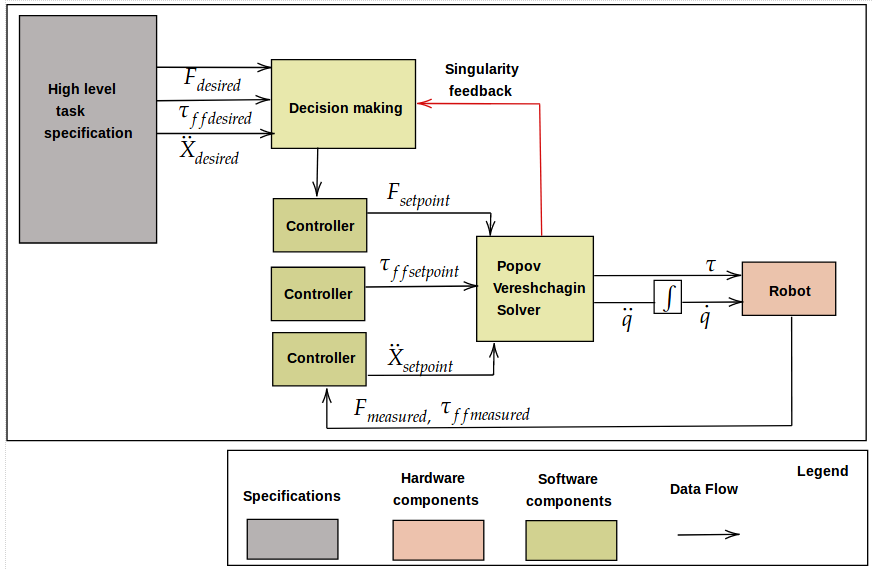
\includegraphics[width=1.0\textwidth]{images/extensionscheme1}
		\caption{Schematic representation of task level specification extension in Popov Vereshchagin solver}
		\label{Controlscheme2}
	\end{figure}
The extension to the current implementation of Popov Vereshchagin solver is given as software proof of concept implementation. This is provided in C++ language. The implementation depends on KDL library \cite{kdl} mentioned earlier. Referring to figure \ref{Controlscheme1} which proposes the original schematic representation of task level specification in Popov Solver. This does not take into account in checking ill conditions for singular configuration. But after providing extension for the above case refer figure \ref{Controlscheme2}, the singularity detection is added as a feedback from the solver to the decision making. In other words, when the solver reaches singular configuration, it is detected and sent as a feedback to the decision making mechanism, which will further exploit this knowledge. Thus achieving separation of concern.

%\subsection{Analysis on constraint coupling matrix}
%The diagnosis for singularity check initiated by analyzing the constraint coupling matrix. Our initial hypothesis is to identify if the kinematic chain can achieve the task constraints mentioned at end effector. This led in identifying the difference between ranks of unit constrained matrix and constraint coupling matrix. 
%\par
%With the knowledge of achievable task constraints, next step is to identify which joint is restricted. Analysis on null space of SVD, leads to the
%%The (right) null space of constraint coupling matrix gives the columns of V corresponding to singular values equal to zero. 
%end result of this process will denotes the direction in which task constraints are achievable. This is an important result, as it indicates the user that the given input task constraint will result in singularity if the constraints are detected as \textit{not achievable}. The solver after extension doe not merely suggest the non achievable constraints, but also indicates  which direction of task constraint results in singularity. 
%\par
%After having implemented the above, the next steps concentrated on how to efficiently perform the calculation, as the matrix inversion involved is very computationally expensive operation. According to the numerical considerations of the constraint coupling matrix refer \ref{Numerical considerations}, we observe that there is a possibility for rank one updates to positive semidefinite matrix (constraint coupling matrix), which satisfy other preconditions such as refer \ref{Decompositions}. Including suggestions from authors in \cite{shakhimardanov2015}, the rank one update of LDL decomposition proposed by \cite{sentana1999econometric} presents an algorithm for updating the positive semi-definite matrix symmetrically after performing a positive rank-one update, which can be applied to matrices which do not have full rank. Based on their proposed algorithm, each rank one update will include only $O(n^2)$ multiplications and additions. This will significantly reduce the computations in the base, where the decomposed form of the constraint coupling matrix is used for solving the linear equation.


\section{Lessons learned}
%\begin{enumerate}
%	\item As mentioned previously , the original solver lacks implementation of run time singularity detection. Given the applied force, it needs to be examined if the kinematic chain is able to generate this force.
%	\item What is the amount of force that can be applied to the kinematic chain without them being felt on joints.
As discussed previously in sections \ref{Numerical considerations} and \ref{Decomposition Techniques}, the evaluation on rank one updates is performed anticipating the performance at the base is less expensive computationally than the existing one, i.e., performing decomposition directly at the base.
\par
The LDL rank one update performed within the inward sweep of solver, will help reduce the computations (see algorithm \ref{alg2}). It indicates that the constraint coupling matrix is obtained in its decomposed form at the base, on further solving for a linear system of equations, it is possible solve for magnitude of constraint forces. This was the initial hypothesis, which was based on also suggestions by \cite{shakhimardanov2015}. Inorder to test this case, the rank one update LDL decomposition was implemented and tested. 
\par
The implementation however did not provide any computationally better procedure for calculating the magnitude of constraint forces. This further led to a comparison between the run time complexities to benchmark for future use.
%	\item We expected rank one update during the loop, compare the ldl decomposition directly at the base, we dont gain any good. We had an expectation that it would but it didnt.
	
%\end{enumerate}
%Idea is based on the point, the equation no 28, at a particular joint you feel the force the end effector force, you project the constraint forces onto the joint space. For the constraint forces we have upto 6 and all of them encode directional information. Linear and angular. Since we know each of the constraints in the end effector. The first vector encodes for eg linear x and the now question is due to see torques in joints due to this force. If none of the joints feel any torque due to the forces then you should be in singular configuration. Its super efficient, this is just one entry of constraint vector, if it zero for all the joints, then we should be able to say that they are singular. 
%In the implementation of the solver, the singular value decomposition is performed on the constraint coupling matrix as the singular values are arranged in descending order as they are decomposed by svd. $\sigma_{1}\geq\sigma_{2}$
%	\item This indicated a check to unsort the svd values.
%	\item https://cseweb.ucsd.edu/classes/wi15/cse252B-a/nullspace.pdf
%	\item 
%	\item By identifying if there are non zero values at the end of each row of the blocked V, we can conclude that the direction of the task constraint can not be achieved.
%	\item According to the numerical considerations of the constraint coupling matrix, we observed that there is a possibility for rank one updates, which satisfy certain preconditions such as \ref{Decompositions}. 
%	\item As suggested by \cite{shakhimardanov2015} the LDL decomposition by \cite{sentana1999econometric} which presents an algorithm for updating the positive semi-definite matrix symmetrically after performing a positive rank-one update, can be applied to matrices which do not have full rank.
%	\item The most important motivation f
	
%	\item The implementation begins by checking if the task constraint can be achieved by the kinematic chain or not.
%	\item By passing user input unit constrained matrix as an argument to the calculation of the magnitude of constraint forces, calculate the rank of the matrix.
%	\item As mentioned earlier, the svd of the constraint coupling matrices provides with matrix of singular values. 
%	\item The difference in rank of unit constrained forces matrix and matrizx with singular values indicate the achievability of the task constraint by the kinematic chain. We now can be sure due to which acceleration constraints i




%\section{Lessons Learned/Drawbacks during implementation}
%epsilon has a special value and close to zero.
%The Sm matrix is being iterated to check the values close to zero. By blocking its changing the view. create a new matrix, copy all the elements into it. What does block function do? It access and projects part of original data.
%Kick out the elements that are non zero rows. Vm block -  sigma is satisfied.
%In vm block , count the number of non zero values in each row. If the all values are zero in a row, then it cannot satisfy that constraint. In non zero cols, its first linear and then angular. (If some of the rows are zero or not).

%/***
%At a particular joint you feel the impact or force applied to the end effector. Project the constraint forces to joint space.
%Unit constrained forces - encode direction information.
%Since we know each entry in A. Suppose it encodes for linear x in first vector, do you see in any of the joints, the torques due to this force. If you do, then its not singular.
%\begin{enumerate}
%	\item We initially begin by analyzing constraint coupling matrix
%\end{enumerate}
